\usetikzlibrary{calc}
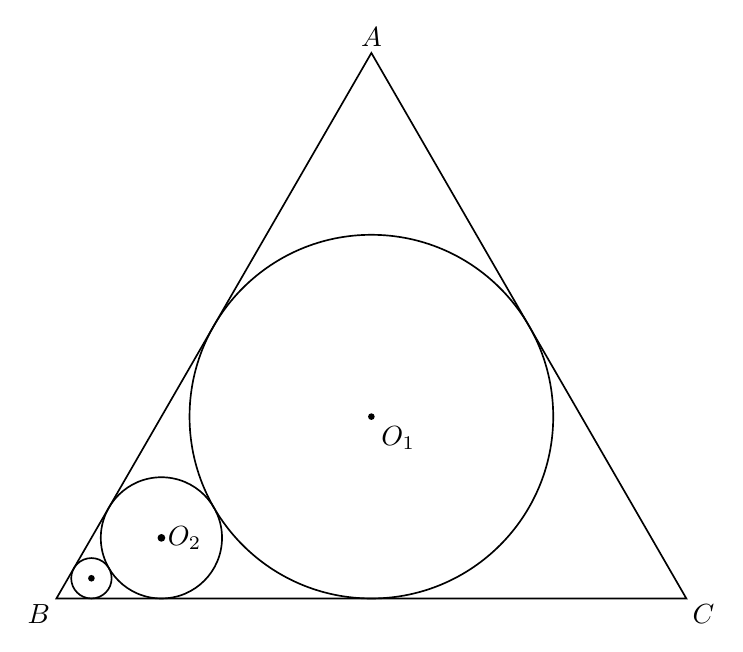
\begin{tikzpicture}[x=1cm,y=1cm,line width=.6pt,font=\normalsize]
\coordinate (B) at (0,0);
\coordinate (C) at (8,0);
\coordinate (A) at (4,6.92820323);
\coordinate (O1) at (4,2.30940108);
\coordinate (O2) at (1.33333333,0.76980036);
\coordinate (O3) at (0.44444444,0.25660012);
\draw (A)--(B)--(C)--cycle;
\draw (O1) circle[radius=2.30940108cm];
\draw (O2) circle[radius=0.76980036cm];
\draw (O3) circle[radius=0.25660012cm];
\fill (O1) circle[radius=1.2pt];
\fill (O3) circle[radius=1.2pt];
\node[above=2pt,inner sep=0pt] at (A) {$A$};
\node[below left=2pt,inner sep=0pt] at (B) {$B$};
\node[below right=2pt,inner sep=0pt] at (C) {$C$};
\node[below right] at (O1) {$O_{1}$};
\node[right=2pt,inner sep=0pt] at (O2) {$O_{2}$};

% Explicit named circle-center points, painted after all region fills.
\fill (O2) circle[radius=1.4pt];
\end{tikzpicture}
